%%%%%%%%%%%%%%%%%%%%%%%%%%%%%%%%%%%%%%%%%%%%%%%%%%%%%%%%%%%%%%%%%%%%%%%%%%%%%%%
\documentclass{article}
\newcommand{\path}{../../assets/settings}
% \input{\path/newcommand.tex}
\input{\path/usepackage.tex}

\usepackage{nopageno} % Paquete para desactivar la numeración de páginas
\title{Resultados Instalacion FV}
\author{Kgnete}
\date{\today}
\begin{document}
\maketitle
%%%%%%%%%%%%%%%%%%%%%%%%%%%%%%%%%%%%%%%%%%%%%%%%%%%%%%%%%
\section*{Disposicion de los paneles}


\subsection*{ Inclinacion  y orientacion de los paneles}



Para la disposición de paneles solares en una cubierta plana, además de las alternativas de orientación Este-Oeste, horizontal, y siguiendo la geometría de la cubierta con inclinación óptima, es importante considerar también la disposición con orientación hacia el sur, que es tradicionalmente la más eficiente en términos de captación de energía solar en el hemisferio norte. A continuación, se presentan las cuatro alternativas junto con una comparativa de sus ventajas y desventajas.

\subsubsection*{Disposición Este-Oeste}
Descripción:
Los paneles se instalan en filas orientadas hacia el Este y el Oeste, con una inclinación moderada (por ejemplo, 10-15 grados).

Ventajas:

    - Maximización del Espacio: Permite una mayor densidad de paneles en la superficie disponible.

    - Producción Distribuida: Genera energía de manera más uniforme a lo largo del día.

    - Menor Sombra: La inclinación moderada reduce las sombras entre las filas de paneles.

Desventajas:

    - Menor Producción Total: Puede resultar en una producción ligeramente inferior a lo largo del año.

    - Complejidad de Instalación: Requiere un diseño más cuidadoso y una estructura de soporte específica.


\subsubsection*{Disposición siguiendo la geometría de la cubierta con Inclinación Óptima}
Descripción:

Los paneles se instalan siguiendo la orientación y la geometría de la cubierta existente, con una inclinación óptima para la localización específica (por ejemplo, 30-35 grados).

Ventajas:

- Aprovechamiento del Espacio: Utiliza eficientemente la superficie disponible, adaptándose a la estructura del techo.

- Maximización de Producción: Optimiza la producción de energía anual, aprovechando al máximo la irradiación solar directa.

- Estética e Integración: Se integra bien con la arquitectura del edificio, mejorando la estética.

Desventajas:

- Sombra: La inclinación puede provocar sombras entre filas si no se gestiona adecuadamente.

- Coste de Instalación: Puede ser más costosa debido a la necesidad de estructuras de soporte adaptadas a la geometría del techo.


\subsubsection*{Disposición Horizontal}
Descripción:

Los paneles se instalan de manera horizontal, directamente sobre la superficie del techo.


Ventajas:

- Facilidad de Instalación: Más sencilla y rápida de instalar, con menos requerimientos estructurales.

- Estética y Viento: Menor impacto visual y resistencia al viento, ya que los paneles están alineados con la cubierta.

- Mantenimiento: Fácil acceso para la limpieza y mantenimiento.

Desventajas:

- Menor Producción: Menor eficiencia debido a la menor captación de luz solar directa y un mayor efecto de la suciedad.

- Desempeño: Produce menos energía en comparación con las disposiciones inclinadas.

\subsubsection*{Disposición Sur con Inclinación Óptima}
Descripción:
Los paneles se instalan orientados hacia el sur, con una inclinación óptima para la localización específica (por ejemplo, 30-35 grados).


Ventajas:

- Máxima Producción: Optimiza la producción de energía anual, aprovechando al máximo la irradiación solar directa.

- Eficiencia: Mayor eficiencia en la captación de luz solar directa durante las horas pico.

Desventajas:

- Espacio: Requiere más espacio entre las filas de paneles para evitar sombras, reduciendo la densidad de paneles por área.

- Sombra: La inclinación mayor puede provocar sombras más largas entre filas, afectando la producción si no se gestiona adecuadamente.


\begin{table}[H]
    \centering
    \setlength{\tabcolsep}{4pt} % Ajusta el espaciado entre columnas
    \renewcommand{\arraystretch}{1.2} % Ajusta el espaciado entre filas
    \begin{tabular}{p{5cm} p{2cm} p{2cm} p{2cm} p{2cm}}
    \toprule
    \textbf{Característica} & \textbf{Este-Oeste} & \textbf{Geometría Cubierta con Inclinación Óptima} & \textbf{Horizontal} & \textbf{Orientación Sur con Inclinación Óptima} \\
    \midrule
    \textbf{Producción de Energía} & Media & Alta & Baja & Muy Alta \\
    \textbf{Uso del Espacio} & Alto & Medio & Alto & Medio \\
    \textbf{Sombra} & Baja & Media & N/A & Alta \\
    \textbf{Facilidad de Instalación} & Media & Baja & Alta & Baja \\
    \textbf{Coste de Instalación} & Medio & Alto & Bajo & Alto \\
    \textbf{Resistencia al Viento} & Media & Media & Alta & Media \\
    \textbf{Mantenimiento} & Media & Media & Alta & Media \\
    \textbf{Distribución de Producción} & Uniforme a lo largo del día & Pico al mediodía & Baja & Pico al mediodía \\
    \textbf{Estética e Integración} & Media & Alta & Baja & Media \\
    \bottomrule
    \end{tabular}
    \caption{Comparativa de Alternativas para la Disposición de Paneles Solares en la Cubierta}
    \label{tab:comparativa}
    \end{table}
    
\subsubsection*{Solución Recomendada}

Recomendación: La elección de la mejor disposición de paneles depende de las prioridades del proyecto:

Máxima Producción Anual: Si el objetivo principal es maximizar la producción de energía, la Alternativa 4: Disposición Sur con Inclinación Óptima es la mejor opción. Aunque requiere más espacio y tiene un costo de instalación más alto, produce la mayor cantidad de energía a lo largo del año.

Optimización del Espacio y Producción Uniforme: Si el espacio es limitado y se busca una producción más uniforme a lo largo del día, la Alternativa 1: Disposición Este-Oeste es adecuada. Esta configuración permite una mayor densidad de paneles y una producción más balanceada.

Estética y Adaptación a la Cubierta: Si se desea aprovechar al máximo la geometría del techo y mejorar la estética del edificio, la Alternativa 2: Disposición siguiendo la geometría de la cubierta con Inclinación Óptima es ideal. Esta opción se integra bien con la arquitectura y maximiza la producción adaptándose a la estructura existente.

Facilidad y Costo de Instalación: Si el presupuesto es limitado y se prefiere una instalación sencilla y resistente, la Alternativa 3: Disposición Horizontal es la mejor opción. Aunque produce menos energía, es más fácil y rápida de instalar, y resiste mejor las condiciones climáticas adversas.

Cada una de estas alternativas tiene sus propias ventajas y desventajas. La selección final debe considerar las condiciones específicas del sitio, el presupuesto disponible y los objetivos energéticos del proyecto.



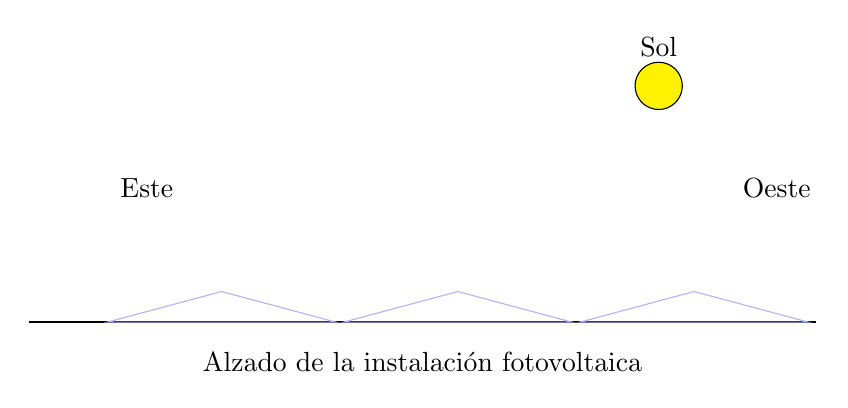
\begin{tikzpicture}
    % Define the angle of inclination
    \def\angle{15}
    \def\height{1.5}
    \def\length{2}
    
    % Function to draw a panel
    \newcommand{\drawpanel}[3]{
        \draw[blue!30] (#1, #2) -- ++(\angle:#3) -- ++(-\angle:#3) -- cycle;
    }

    % Draw the ground line
    \draw[thick] (0,0) -- (10,0);
    
    % Draw the panels facing east
    \foreach \x in {1, 4, 7} {
        \drawpanel{\x}{0}{\height}
    }
    
    % Labels for east and west
    \node at (1.5, 1.7) {Este};
    \node at (9.5, 1.7) {Oeste};

    % Label the title
    \node at (5, -0.5) {Alzado de la instalación fotovoltaica};

    % Draw the sun for reference
    \draw[fill=yellow] (8,3) circle (0.3);
    \node at (8,3.5) {Sol};
    
    % Draw arrows to indicate sun path
    % \draw[->,thick] (8,3) -- (7,1.5);
    % \draw[->,thick] (2,3) -- (3,1.5);
\end{tikzpicture}



\subsection*{Inversor}


Comparativa de Alternativas de Inversores para una Instalación Fotovoltaica de 30 kW en una Cubierta Plana con Obstáculos
Alternativas de Inversores Consideradas:
Inversores Centrales
Inversores String
Microinversores
1. Inversores Centrales
Descripción:
Un solo inversor central maneja la conversión de corriente continua (CC) a corriente alterna (CA) para toda la instalación.

Ventajas:

Coste: Menor coste por vatio comparado con otras alternativas.
Mantenimiento: Mantenimiento centralizado y más sencillo.
Eficiencia: Alta eficiencia en la conversión de energía.
Desventajas:

Sombra y Obstáculos: Menor tolerancia a sombras y obstáculos, ya que el rendimiento del sistema puede verse afectado por el bajo rendimiento de un solo panel.
Flexibilidad: Menos flexible en términos de diseño y expansión futura.
Fallos: Un fallo en el inversor puede detener la producción de energía de toda la instalación.
2. Inversores String
Descripción:
Múltiples inversores en serie (strings) manejan la conversión de CC a CA de grupos de paneles.

Ventajas:

Coste Moderado: Más económico que los microinversores pero más caro que los inversores centrales.
Flexibilidad: Mejor gestión de sombras y obstáculos comparado con los inversores centrales.
Mantenimiento: Mantenimiento aún centralizado, pero más modular que los inversores centrales.
Desventajas:

Sombra y Obstáculos: Aún susceptible a problemas de sombra, aunque mejor que los inversores centrales.
Eficiencia: Menor eficiencia comparado con inversores centrales, especialmente en condiciones no ideales.
Complejidad: Mayor complejidad en el cableado y diseño comparado con inversores centrales.
3. Microinversores
Descripción:
Cada panel solar tiene su propio microinversor que convierte CC a CA directamente en el panel.

Ventajas:

Sombra y Obstáculos: Mayor tolerancia a sombras y obstáculos, ya que cada panel opera independientemente.
Flexibilidad: Máxima flexibilidad en el diseño y fácil expansión futura.
Eficiencia: Mayor eficiencia en sistemas con condiciones variables (sombra, orientación, etc.).
Fallos: Un fallo en un microinversor afecta solo a un panel, no a toda la instalación.
Desventajas:

Coste: Mayor coste inicial por vatio.
Mantenimiento: Más puntos de fallo potenciales y mantenimiento distribuido puede ser más complejo.
Resistencia: Expuestos a las condiciones climáticas y pueden necesitar más protección.

Comparativa de Alternativas


\begin{table}[h]
\centering
\begin{tabular}{lccc}
\toprule
\textbf{Característica} & \textbf{Inversores Centrales} & \textbf{Inversores String} & \textbf{Microinversores} \\
\midrule
Coste Inicial & Bajo & Medio & Alto \\
Mantenimiento & Centralizado & Modular & Distribuido \\
Eficiencia & Alta & Media & Alta \\
Flexibilidad de Diseño & Baja & Media & Alta \\
Gestión de Sombra & Baja & Media & Alta \\
Facilidad de Expansión & Baja & Media & Alta \\
Resiliencia a Fallos & Baja & Media & Alta \\
Complejidad del Sistema & Baja & Media & Alta \\
\bottomrule
\end{tabular}
\caption{Comparativa de Alternativas de Inversores}
\label{tab:comparativa_inversores}
\end{table}


\subsubsection*{Recomendación}
Microinversores son recomendados para la instalación en una cubierta plana con obstáculos, debido a su alta tolerancia a sombras y obstáculos, mayor flexibilidad de diseño, y mayor eficiencia en condiciones variables. Aunque el coste inicial es mayor, la resiliencia a fallos y la facilidad de expansión futura los hacen una inversión adecuada para optimizar la producción de energía en un entorno desafiante.

Sin embargo, si el presupuesto es una restricción significativa, los inversores string pueden ser una alternativa viable, ofreciendo un equilibrio entre coste y rendimiento. Los inversores centrales se recomendarían solo en casos donde el coste inicial sea el factor determinante y las sombras u obstáculos no sean un problema significativo.




% \begin{thebibliography}{9}
%     \bibitem{1}
%     fsadf
%     \bibitem{2}
%     fasdfasd
% \end{thebibliography}

\end{document}
